\chapter{Hardware Abstraction Layer}
\label{chap_hal}

Hardware Abstraction Layer (HAL) berfungsi mengabstraksi hardware dan menyediakan layanan-layanan yang sama terlepas dari paltform hardware yang digunakan. HAL dapat dianalogikan seperti \emph{device driver} pada sistem komputer PC karena akan berhubungan langsung dengan hardware. Tabel \ref{tabel-func-hal} menampilkan antarmuka yang disediakan HAL untuk digunakan oleh modul-modul lainnya.

\begin{table}[h]
  \centering
  \begin{tabular}{|m{5cm}|m{8cm}|}
    \hline
    \bf{Nama Fungsi} & \bf{Kegunaan} \\
    \hline
    HW Init & Menginisialisasi Hardware \\
    \hline
    IO Receive & Menerima 1 byte data melalui port IO \\
    \hline
    IO Transmit & Mengirimkan 1 byte data melalui port IO \\
    \hline
    Memory Internal Read & Membaca 1 byte data dari internal memory \\
    \hline
    Memory Internal Write & Menulis 1 byte data dari internal memory \\
    \hline
    Memory Eksternal Read & Membaca 1 byte data dari external memory \\
    \hline
    Memory Eksternal Write & Menulis 1 byte data dari external memory \\
    \hline
  \end{tabular}
  \caption{Daftar antarmuka fungsi yang disediakan HAL}
  \label{tabel-func-hal}
\end{table}

\section{HW Init}
\label{sec_hwinit}

Berfungsi mempersiapkan HW untuk menyediakan layanan bagi modul-modul lainnya. Gambar \ref{fig-dfd-hwinit} menampilkan DFD dari fungsi HW Init. Implementasi dari Fungsi ini sangat bergantung pada platform smartcard yang akan digunakan. 

\begin{figure}[!h]
\centering
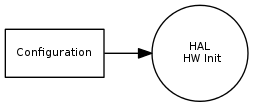
\includegraphics[width=0.5\textwidth]{image/hal/dfd_hwinit.png}
\caption{DFD HW Init}
\label{fig-dfd-hwinit}
\end{figure}

\begin{figure}[!h]
\centering
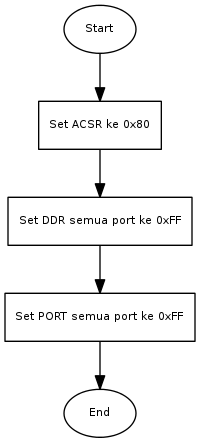
\includegraphics[height=0.5\textheight]{image/hal/flow_hwinit.png}
\caption{Flowchart HW Init}
\label{fig-flow-hwinit}
\end{figure}

Gambar \ref{fig-flow-hwinit} menampilkan diagram alir fungsi HW Init pada smartcard berbasis funcard (uC AT90S8515 \and EEPROM 24C64).

Pertama fungsi hw init akan menginisialisasi pin ke 6 dari port B dari mikrokontroler sebagai port Output dengan men-set Data Direction Register (DDR) 0x40, dan menginisialisasi nilainya menjadi 1 (high) dengan men-set Data Register (PORTB) menjadi 0x40.

Selanjutnya fungsi ini akan mematikan modul Analog Comparator pada mikrokontroler dengan tujuan mengurangi konsumsi daya dengan mengeset bit ke-7 (ACD - Analog Comparator Disable) dari ACSR (Analog Comparator Control and Status Register). 

\subsection {Pengujian}

\begin{table}[h]
  \centering
  \begin{tabular}{ | c | }
    \hline
    \bf{Output} \\
    \hline
    DDRB = 0x40 \\
    PORTB = 0x40 \\
    ACSR = 0x80 \\
    \hline
  \end{tabular}
  \caption{Test Vector Fungsi HAL HW Init}
  \label{tabel-test-hwinit}
\end{table}

Tabel \ref{tabel-test-hwinit} menampilkan Test Vector yang digunakan untuk menguji fungsi HAL HW Init.

\subsection {Implementasi}

Tabel \ref{tabel-hwinit} menampilkan purwarupa dari implementasi fungsi HAL HW Init. 

\begin{table}[!h]
  \centering
  \begin{tabular}{p{2cm} p{8cm}}
    \hline\\
    {\bf Name} & HAL\_HWInit\\
    \hline\\
    {\bf Input} & -
    \\
    \hline\\
    {\bf Output} & -
    \\
    \hline
  \end{tabular}
  \caption{Prototype Fungsi HW Init}
  \label{tabel-hwinit}
\end{table}

Listing \ref{list-hwinit} menampilkan potongan program yang mengimplementasi fungsi HAL HW Init.

\begin{lstlisting}[caption={Listing Program Fungsi HAL HW Init}, label={list-hwinit}]
void HAL_HWInit()
{
	outb(DDRB ,0x40);
	outb(PORTB,0x40);
	outb(ACSR ,0x80);
}
\end{lstlisting}

\section{IO Receive Byte T0}
\label{sec_rxbytet0}

Berfungsi menerima 1 byte data dari Port IO menggunakan protokol komunikasi T0. Gambar \ref{fig-dfd-rxbytet0} menampilkan DFD dari fungsi HAL IO Receive Byte T0(RxByte). Implementasi dari Fungsi ini sangat bergantung pada platform smartcard dimana pintarOS akan digunakan. Gambar \ref{fig-flow-rxbytet0} menampilkan diagram alir dari fungsi Receive Byte T0 untuk \emph{smart card} funcard.

\begin{figure}[!h]
\centering
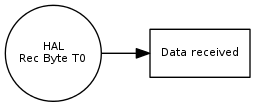
\includegraphics[width=0.5\textwidth]{image/hal/dfd_rxbytet0.png}
\caption{DFD Receive Byte T0}
\label{fig-dfd-rxbytet0}
\end{figure}

\begin{figure}[!h]
\centering
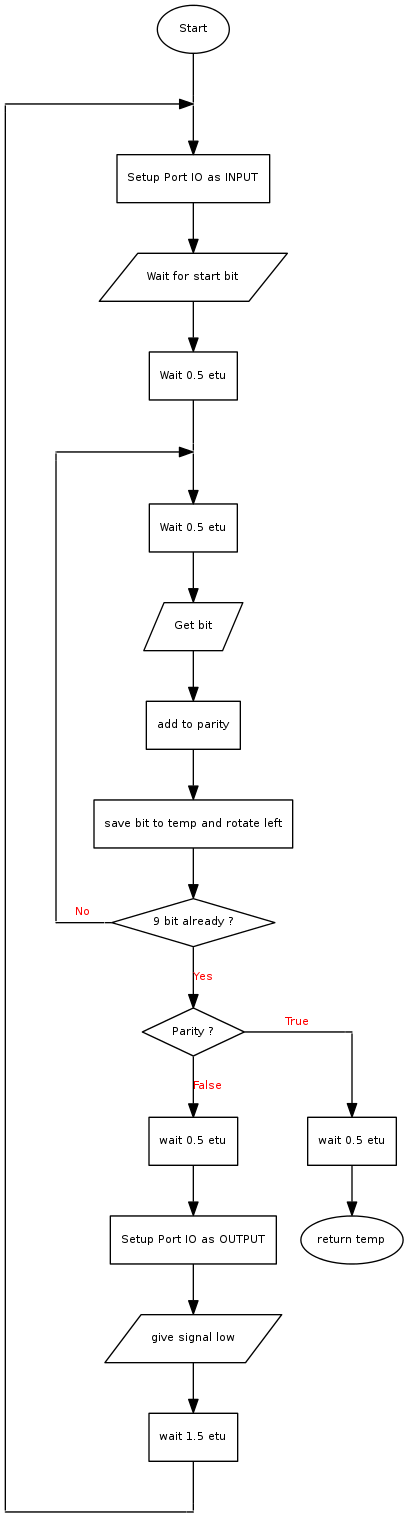
\includegraphics[height=0.9\textheight]{image/hal/flow_rxbytet0.png}
\caption{Flowchart Receive Byte T0}
\label{fig-flow-rxbytet0}
\end{figure}

\subsection {Pengujian}

\begin{table}[h]
  \centering
  \begin{tabular}{ | c || c | }
    \hline
    \bf{Input}  & \bf{Output} \\
    \hline
    \bf{Databyte (from terminal)} & \bf{Return Value}\\
    \hline
    0x00 & = 0x00 \\
    0x01 & = 0x01 \\
    \hline
    \multicolumn{2}{ |c| }{...} \\
    \multicolumn{2}{ |c| }{...} \\
    \hline
    0xff & = 0xff \\
    \hline
  \end{tabular}
  \caption{Test Vector Fungsi HAL Receive Byte T0}
  \label{tabel-test-rxbytet0}
\end{table}

Tabel \ref{tabel-test-getbyte} menampilkan Test Vector yang digunakan untuk menguji fungsi HAL Receive Byte T0.

\subsection {Implementasi}

Tabel \ref{tabel-rxbytet0} menampilkan purwarupa dari implementasi fungsi HAL IO Receive Byte T0. 

\begin{table}[!h]
  \centering
  \begin{tabular}{p{2cm} p{8cm}}
    \hline\\
    {\bf Name} & HAL\_IO\_RxByteT0\\
    \hline\\
    {\bf Input} & -
    \\
    \hline\\
    {\bf Output} & data yang diterima (1 byte)
    \\
    \hline
  \end{tabular}
  \caption{Prototype Fungsi HAL IO Receive Byte T0}
  \label{tabel-rxbytet0}
\end{table}

Listing \ref{list-rxbytet0} menampilkan potongan program yang mengimplementasi fungsi HAL IO Receive Byte.

\begin{lstlisting}[language={[x86masm]Assembler}, caption={Listing Program Fungsi HAL IO Receive Byte T0}, label={list-rxbytet0}]
;========================================================================
; Receive a byte with T=0 error correction.
; result r25(=0):r24
HAL_IO_RxByteT0:
	push	r23				; 2 - getbit
	push	r22				; 2 - delay
	push	r21				; 2 - loop counter
	push	r20				; 2 - parity counter

	; Set direction bit, to indicate, that we received a byte
	ldi		r22, 1
	sts		direction,r22

restartrecbyte:
	; Setup IN direction
	cbi		DDRB, 6			; 2
	cbi		PORTB, 6		; 2

; Wait for start bit.
waitforstart:
	; Bit begins here.
	sbic	PINB, IO_PIN	; 1/2!
	rjmp	waitforstart	; 2/0
	sbic	PINB, IO_PIN	; 1/2! - Recheck for spike
	rjmp	waitforstart	; 2/0
	; Sample start bit
	clr		r24				; 1
	clr		r25				; 1 - Clear zero byte for ADC
	ldi		r22, 31			; 1
	rcall	delay			; 100
	rcall	getbit			; 3 (16bit PC)
	;brcs	waitforstart	; 1/2 - Go on, even if not valid a start bit?
	nop						; 1 - For brcs
; Receive now 9 bits
	ldi		r21, 0x09		; 1
	clr		r20				; 1
	ldi		r22, 66			; 1
	nop						; 1
	nop						; 1
rnextbit:
	rcall	delay			; 205/202
	rcall	getbit			; 3
	add		r20, r23		; 1
	clc						; 1
	sbrc	r23, 0			; 1/2
	sec						; 1/0
	ror		r24				; 1
	ldi		r22, 65			; 1
	dec		r21				; 1
	brne	rnextbit		; 1/2
; Check parity
	rol		r24				; 1 - We've rotated one to much
	sbrc	r20, 0			; 1/2
	rjmp	regetbyte		; 2/0

	; Wait halve etu
	ldi		r22, 76			; 1
	rcall	delay			; 235 - Precise enough

	clr		r25
	pop		r20				; 2 - parity counter
	pop		r21				; 2 - loop counter
	pop		r22				; 2 - delay
	pop		r23				; 2 - getbit
	ret

regetbyte:
	; Wait halve etu
	ldi		r22, 76			; 1
	rcall	delay			; 235 - Precise enough
	; Set OUT direction
	sbi		DDRB, 6			; 2
	; Signal low
	cbi		PORTB, 6		; 2
	ldi		r22, 182		; 2
	rcall	delay			; 553 - about 1.5 etu
	rjmp	restartrecbyte	; 2

;========================================================================
; Read a bit.
; Uses r23, r25
; Returns bit in r23.0.
; 5 cycles before first bit
; 8 cycles after last bit.
getbit:
	clr		r23				; 1
	clc						; 1
	; At start + 112 cycles
	sbic	PINB, IO_PIN	; 1/2
	sec						; 1/0
	adc		r23, r25		; 1
	rcall	intrabitdelay	; 70
	clc						; 1
	; At start + 186 cycles
	sbic	PINB, IO_PIN	; 1/2
	sec						; 1/0
	adc		r23, r25		; 1
	rcall	intrabitdelay	; 70
	clc						; 1
	; At start + 260 cycles
	sbic	PINB, IO_PIN	; 1/2
	sec						; 1/0
	adc		r23, r25		; 1
	; Get second bit of the sum.
	lsr		r23				; 1
	ret						; 4	(with 16bit PC)
\end{lstlisting}

\section{IO Transmit Byte T0}
\label{sec_txbytet0}

Berfungsi mengirimkan 1 byte data melalui Port IO menggunakan protokol komunikasi T0. Gambar \ref{fig-dfd-txbytet0} menampilkan DFD dari fungsi HAL IO Transmit Byte T0(RxByte). Gambar \ref{fig-flow-txbytet0} menampilkan diagram alir dari fungsi Transmit Byte T0 untuk \emph{smart card} funcard.

\begin{figure}[!h]
\centering
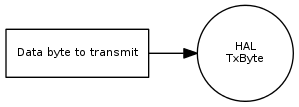
\includegraphics[width=0.5\textwidth]{image/hal/dfd_txbytet0.png}
\caption{DFD Transmit Byte T0}
\label{fig-dfd-txbytet0}
\end{figure}

\begin{figure}[!h]
\centering
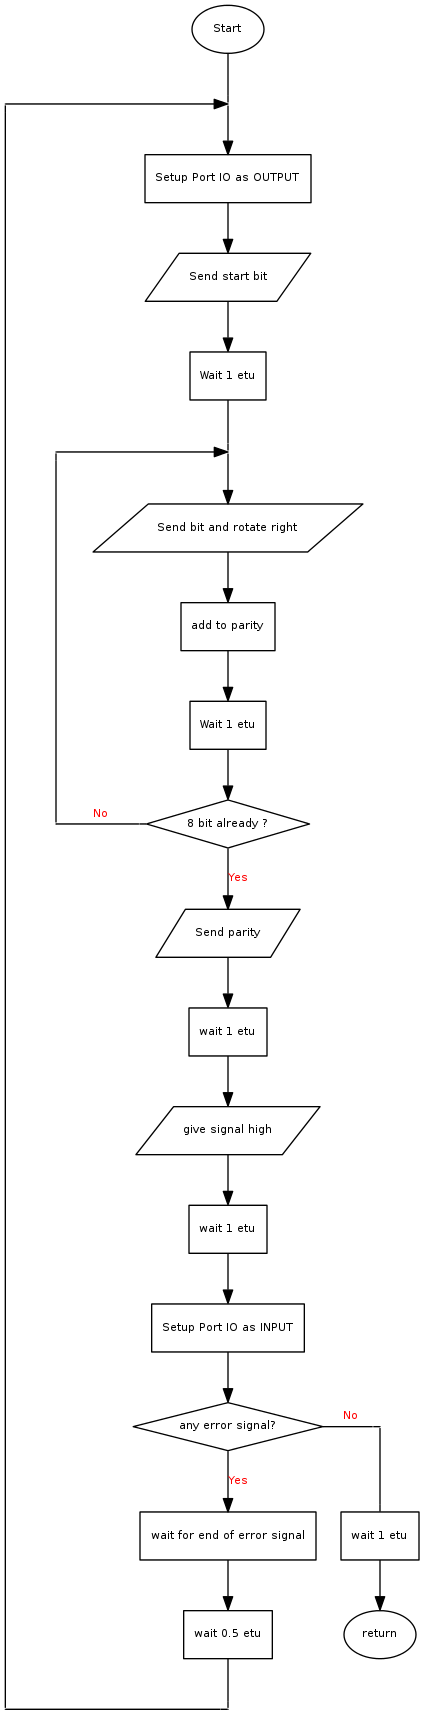
\includegraphics[height=0.9\textheight]{image/hal/flow_txbytet0.png}
\caption{Flowchart HAL IO Transmit Byte T0}
\label{fig-flow-txbytet0}
\end{figure}

\subsection {Pengujian}

\begin{table}[h]
  \centering
  \begin{tabular}{ | c || c | }
    \hline
    \bf{Input}  & \bf{Output} \\
    \hline
    \bf{Data} & \bf{Databyte (to terminal)}\\
    \hline
    0x00 & = 0x00 \\
    0x01 & = 0x01 \\
    \hline
    \multicolumn{2}{ |c| }{...} \\
    \multicolumn{2}{ |c| }{...} \\
    \hline
    0xff & = 0xff \\
    \hline
  \end{tabular}
  \caption{Test Vector Fungsi HAL IO Transmit Byte T0}
  \label{tabel-test-txbytet0}
\end{table}

Tabel \ref{tabel-test-txbytet0} menampilkan Test Vector yang digunakan untuk menguji fungsi HAL IO Transmit Byte T0.

\subsection {Implementasi}

Tabel \ref{tabel-txbytet0} menampilkan purwarupa dari implementasi fungsi HAL IO Transmit Byte T0. 

\begin{table}[!h]
  \centering
  \begin{tabular}{p{2cm} p{8cm}}
    \hline\\
    {\bf Name} & HAL\_TxByteT0\\
    \hline\\
    {\bf Input} & data yang akan dikirimkan (1 byte)
    \\
    \hline\\
    {\bf Output} & -
    \\
    \hline
  \end{tabular}
  \caption{Prototype Fungsi HAL IO Transmit Byte T0}
  \label{tabel-txbytet0}
\end{table}

Listing \ref{list-txbytet0} menampilkan potongan program yang mengimplementasi fungsi HAL IO Transmit Byte T0.

\begin{lstlisting}[language={[x86masm]Assembler}, caption={Listing Program Fungsi HAL IO Transmit Byte T0}, label={list-txbytet0}]
;========================================================================
; Send a byte with T=0 error correction.
; byte r25(=0):r24
HAL\_TxByteT0:
	push	r22				; 2 - delay
	push	r23				; 2 - parity counter

	lds		r22,direction
	tst		r22
	breq	resendbytet0
	rcall	delay1etu		;
	rcall	delay1etu		;
	; Clear direction bit, to indicate, that we sent a byte
	ldi		r22, 0
	sts		direction,r22

resendbytet0:
	; Set OUT direction
	sbi		PORTB, 6		; 2
	sbi		DDRB, 6			; 2
	; Send start bit
	cbi		PORTB, IO_PIN	; 2
	ldi		r22, 119		; 1
	rcall	delay			; 364
	; Send now 8 bits
	ldi		r25, 0x08		; 1
	clr		r23				; 1
snextbit:
	ror		r24				; 1
	brcs	sendbit1		; 1/2
	cbi		PORTB, IO_PIN	; 2
	rjmp	bitset			; 2
sendbit1:
	sbi		PORTB, IO_PIN	; 2
	inc		r23				; 1
bitset:
	ldi		r22, 118		; 1
	rcall	delay			; 361
	nop						; 1
	dec		r25				; 1
	brne	snextbit		; 1/2
	; Send parity
	sbrc	r23, 0			; 1/2
	rjmp	sendparity1		; 2
	nop						; 1
	nop						; 1
	cbi		PORTB, IO_PIN	; 2
	rjmp	delayparity		; 2
sendparity1:
	nop						; 1
	sbi		PORTB, IO_PIN	; 2
	nop						; 1
	nop						; 1
delayparity:
	ldi		r22, 112		; 1
	rcall	delay			; 343
	; Stop bit
	sbi		PORTB, IO_PIN	; 2
	ldi		r22, 119		; 1
	rcall	delay			; 364
	; Set IN direction
	cbi		DDRB, 6			; 2
	cbi		PORTB, 6		; 2
	; Look for error signal
	clc						; 1
	sbic	PINB, IO_PIN	; 1/2
	sec						; 1/0
	brcs	retsendbytet0	; 1/2
	; Resend byte
	; Bring byte to starting position
	ror		r24				; 1
	; Wait for end of error signal
waitforendoferror:
	sbic	PINB, IO_PIN	; 1/2!
	rjmp	waitforendoferror	; 2/0
	; Wait then a halve etu
	ldi		r22, 58			; 1
	rcall	delay			; 181
	rjmp	resendbytet0	; 2
	; return
retsendbytet0:
	ldi		r22, 116		; 1
	rcall	delay			; 355
	pop		r23				; 2 - parity counter
	pop		r22				; 2 - delay
	ret						; 4
;========================================================================
\end{lstlisting}

\section{Internal Memory Read Byte}
\label{sec_internalmemoryreadbyte}

Berfungsi membaca 1 byte data dari Memory EEPROM Internal. Gambar \ref{fig-dfd-internalreadbyte} menampilkan DFD dari fungsi HAL Internal Memory Read Byte (ReadByte). 

\begin{figure}[!h]
\centering
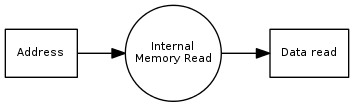
\includegraphics[width=0.75\textwidth]{image/hal/dfd_internalreadbyte.png}
\caption{DFD Internal Memory Read Byte}
\label{fig-dfd-internalreadbyte}
\end{figure}

\begin{figure}[!h]
\centering
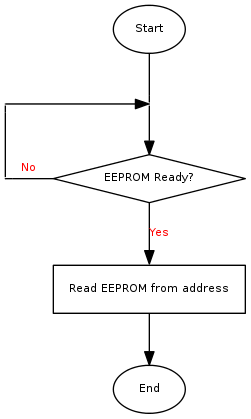
\includegraphics[height=0.4\textheight]{image/hal/flow_internalreadbyte.png}
\caption{Flowchart Internal Memory Read Byte}
\label{fig-flow-internalreadbyte}
\end{figure}

\subsection {Pengujian}

\begin{table}[!h]
  \centering
  \begin{tabular}{ | c || c | }
    \hline
    \bf{Input}  & \bf{Output} \\
    \hline
    \bf{address} & \bf{Return Value}\\
    \hline
    \multicolumn{2}{ |c| }{Filled internal memory according to their address} \\
    \multicolumn{2}{ |c| }{} \\
    \multicolumn{2}{ |c| }{
      \begin{tabular}{ c | c | }
        \cline{2-2}
        0x000 - 0x00f & 0x00, 0x01, ..., 0x0f \\
        \cline{2-2}
        0x010 - 0x01f & 0x10, 0x11, ..., 0x1f \\
        \cline{2-2}
        & ... \\
        \cline{2-2}
        0x0f0 - 0x0ff & 0xf0, 0xf1, ..., 0xff \\
        \cline{2-2}
        & ... \\
        \cline{2-2}
        0x100 - 0x1ff & 0x00, 0x01, ..., 0xff \\
        \cline{2-2}
      \end{tabular}
    } \\
    \multicolumn{2}{ |c| }{} \\

    \hline
    0x000 & = 0x00 \\
    0x001 & = 0x01 \\
    \hline
    \multicolumn{2}{ |c| }{...} \\
    \hline
    0x0ff & = 0xff \\
    0x100 & = 0x00 \\
    0x101 & = 0x01 \\
    \hline
    \multicolumn{2}{ |c| }{...} \\
    \hline
    0x1ff & = 0xff \\
    \hline
  \end{tabular}
  \caption{Test Vector Fungsi HAL Memory Internal Read Byte}
  \label{tabel-test-internalreadbyte}
\end{table}

Tabel \ref{tabel-test-internalreadbyte} menampilkan Test Vector yang digunakan untuk menguji fungsi HAL Memory Internal Read Byte.

\subsection {Implementasi}

Tabel \ref{tabel-internalreadbyte} menampilkan purwarupa dari implementasi fungsi HAL Memory Internal Read Byte. 

\begin{table}[!h]
  \centering
  \begin{tabular}{p{2cm} p{8cm}}
    \hline\\
    {\bf Name} & HAL\_InternalReadByte\\
    \hline\\
    {\bf Input} & alamat memory yang akan dibaca
    \\
    \hline\\
    {\bf Output} & data hasil pembacaan (1 byte)
    \\
    \hline
  \end{tabular}
  \caption{Prototype Fungsi HAL Internal Memory Read Byte}
  \label{tabel-internalreadbyte}
\end{table}

Listing \ref{list-internalreadbyte} menampilkan potongan program yang mengimplementasi fungsi HAL Memory Internal Read Byte.

\begin{lstlisting}[caption={Listing Program Fungsi HAL Memory Internal Read Byte}, label={list-internalreadbyte}]
uint8_t HAL_InternalReadByte(const uint8_t * addr)
{
  while(!eeprom_is_ready());

  return eeprom_read_byte(addr);
}
\end{lstlisting}

\section{Internal Memory Write Byte}
\label{sec_internalmemorywritebyte}

Berfungsi menulis 1 byte data ke Memory EEPROM Internal. Gambar \ref{fig-dfd-internalwritebyte} menampilkan DFD dari fungsi HAL Internal Memory Write Byte. 

\begin{figure}[!h]
\centering
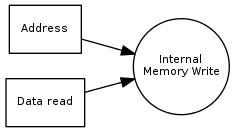
\includegraphics[width=0.5\textwidth]{image/hal/dfd_internalwritebyte.png}
\caption{DFD Internal Memory Write Byte}
\label{fig-dfd-internalwritebyte}
\end{figure}

\begin{figure}[!h]
\centering
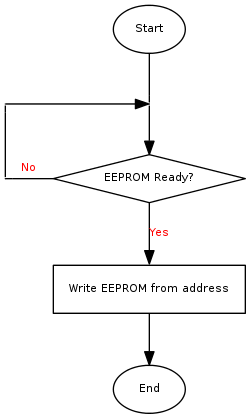
\includegraphics[height=0.4\textheight]{image/hal/flow_internalwritebyte.png}
\caption{Flowchart Internal Memory Write Byte}
\label{fig-flow-internalwritebyte}
\end{figure}

\subsection {Pengujian}

\begin{table}[!h]
  \centering
  \begin{tabular}{ | c | c || c | }
    \hline
    \multicolumn{2}{ |c|| }{\bf{Input}}  & \bf{Output} \\
    \hline
    \bf{address} & \bf{data} & \bf{Memory value @address}\\
    0x000 & 0x00 & = 0x00 \\
    \hline
    \multicolumn{3}{ |c|| }{...}\\
    \hline
    0x00f & 0x0f & = 0x0f \\
    0x010 & 0x10 & = 0x10 \\
    \hline
    \multicolumn{3}{ |c|| }{...}\\
    \hline
    0x01f & 0x1f & = 0x1f \\
    \hline
    \multicolumn{3}{ |c|| }{...}\\
    \hline
    0x0ff & 0xff & = 0xff \\
    0x100 & 0x00 & = 0x00 \\
    \hline
    \multicolumn{3}{ |c|| }{...}\\
    \hline
    0x1ff & 0xff & = 0xff \\
    \hline
  \end{tabular}
  \caption{Test Vector Fungsi HAL Memory Internal Write Byte}
  \label{tabel-test-internalwritebyte}
\end{table}

Tabel \ref{tabel-test-internalwritebyte} menampilkan Test Vector yang digunakan untuk menguji fungsi HAL Memory Internal Write Byte.

\subsection {Implementasi}

Tabel \ref{tabel-internalwritebyte} menampilkan purwarupa dari implementasi fungsi HAL Memory Internal Write Byte. 

\begin{table}[!h]
  \centering
  \begin{tabular}{p{2cm} p{8cm}}
    \hline\\
    {\bf Name} & HAL\_InternalWriteByte\\
    \hline\\
    {\bf Input} & 
    \begin{itemize}[noitemsep,topsep=0pt,parsep=0pt,partopsep=0pt]
    \item alamat memory yang akan ditulis
    \item data yang akan ditulis (1 byte)
    \end{itemize}
    \\
    \hline\\
    {\bf Output} & -
    \\
    \hline
  \end{tabular}
  \caption{Prototype Fungsi HAL Internal Memory Write Byte}
  \label{tabel-internalwritebyte}
\end{table}

Listing \ref{list-internalwritebyte} menampilkan potongan program yang mengimplementasi fungsi HAL Memory Internal Write Byte.

\begin{lstlisting}[caption={Listing Program Fungsi HAL Memory Internal Write Byte}, label={list-internalwritebyte}]
void HAL_InternalWriteByte(uint8_t * addr, uint8_t byte)
{
  while(!eeprom_is_ready());

  return eeprom_write_byte(addr, byte);
}
\end{lstlisting}

\section{External Memory Read Byte}
\label{sec_externalmemoryreadbyte}

Berfungsi membaca 1 byte data dari Memory EEPROM Eksternal.

Gambar \ref{fig-dfd-externalreadbyte} menampilkan DFD dari fungsi HAL External Memory Read Byte. 

\begin{figure}[!h]
\centering
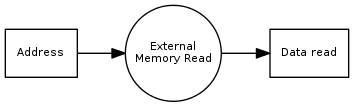
\includegraphics[width=0.75\textwidth]{image/hal/dfd_externalreadbyte.png}
\caption{DFD External Memory Read Byte}
\label{fig-dfd-externalreadbyte}
\end{figure}

%% \begin{figure}[!h]
%% \centering
%% \includegraphics[height=0.4\textheight]{image/hal/flow_externalreadbyte.png}
%% \caption{Flowchart External Memory Read Byte}
%% \label{fig-flow-externalreadbyte}
%% \end{figure}

\subsection {Pengujian}

\begin{table}[!h]
  \centering
  \begin{tabular}{ | c || c | }
    \hline
    \bf{Input}  & \bf{Output} \\
    \hline
    \bf{address} & \bf{Return Value}\\
    \hline
    \multicolumn{2}{ |c| }{Filled external memory according to their address} \\
    \multicolumn{2}{ |c| }{} \\
    \multicolumn{2}{ |c| }{
      \begin{tabular}{ c | c | }
        \cline{2-2}
        0x00000 - 0x000ff & {[0x00, 0x01, ..., 0xff]} \\
        \cline{2-2}
        & ... \\
        \cline{2-2}
        0x00100 - 0x00fff & {[0x00, 0x01, ..., 0xff]x 0xE} \\
        \cline{2-2}
        & ... \\
        \cline{2-2}
        0x01000 - 0x0ffff & {[0x00, 0x01, ..., 0xff]x 0xEF} \\
        \cline{2-2}
        & ... \\
        \cline{2-2}
        0x10000 - 0xfffff & {[0x00, 0x01, ..., 0xff]x 0xEFF} \\
        \cline{2-2}
      \end{tabular}
    } \\
    \multicolumn{2}{ |c| }{} \\

    \hline
    0x00000 & = 0x00 \\
    0x00001 & = 0x01 \\
    \hline
    \multicolumn{2}{ |c| }{...} \\
    \hline
    0x000ff & = 0xff \\
    0x00100 & = 0x00 \\
    \hline
    \multicolumn{2}{ |c| }{...} \\
    \hline
    0x00fff & = 0xff \\
    0x01000 & = 0x00 \\
    \hline
    \multicolumn{2}{ |c| }{...} \\
    \hline
    0x0ffff & = 0xff \\
    0x10000 & = 0x00 \\
    \hline
    \multicolumn{2}{ |c| }{...} \\
    \hline
    0xfffff & = 0xff \\
    \hline
  \end{tabular}
  \caption{Test Vector Fungsi HAL Memory External Read Byte}
  \label{tabel-test-internalreadbyte}
\end{table}

Tabel \ref{tabel-test-internalreadbyte} menampilkan Test Vector yang digunakan untuk menguji fungsi HAL Memory External Read Byte.

\subsection {Implementasi}

Tabel \ref{tabel-externalreadbyte} menampilkan purwarupa dari implementasi fungsi HAL Memory External Read Byte.

\begin{table}[!h]
  \centering
  \begin{tabular}{p{2cm} p{8cm}}
    \hline\\
    {\bf Name} & HAL\_ExternalReadByte\\
    \hline\\
    {\bf Input} & alamat memory yang akan dibaca
    \\
    \hline\\
    {\bf Output} & data hasil pembacaan (1 byte)
    \\
    \hline
  \end{tabular}
  \caption{Prototype Fungsi HAL External Memory Read Byte}
  \label{tabel-externalreadbyte}
\end{table}

Listing \ref{list-externalreadbyte} menampilkan potongan program yang mengimplementasi fungsi HAL Memory External Read Byte.

\begin{lstlisting}[language={[x86masm]Assembler}, caption={Listing Program Fungsi HAL Memory External Read Byte}, label={list-externalreadbyte}]
; address r25:r24 
; result r25(=0):r24
HAL_ExternalReadByte:
	push	r31
	push	r30
	push	r19
	push	r18
	push	r16
	push	r1
	push	r0
	mov	r31,r25
	mov	r30,r24
; Start
	rcall	xereadlocal
; Done
	clr	r25
	mov	r24,r0
	pop	r0
	pop	r1
	pop	r16
	pop	r18
	pop	r19
	pop	r30
	pop	r31
	ret

; address r31:r30 
; result r0 = XE(Z+)
xereadlocal:
	rcall	XEAddr
	rcall	XEStrt
	clc
	ldi		r19,0xA1
	rcall	XEEOut
	rcall	XE0Bit
	rcall	XEEIn
	rcall	XE1Bit
	rcall	XEStop
	ret
\end{lstlisting}

\section{External Memory Write Byte}
\label{sec_externalmemorywritebyte}

Berfungsi menulis 1 byte data ke Memory EEPROM External. Gambar \ref{fig-dfd-externalwritebyte} menampilkan DFD dari fungsi HAL External Memory Write Byte. 

\begin{figure}[!h]
\centering
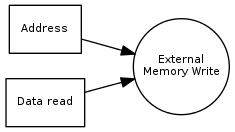
\includegraphics[width=0.5\textwidth]{image/hal/dfd_externalwritebyte.png}
\caption{DFD External Memory Write Byte}
\label{fig-dfd-externalwritebyte}
\end{figure}

\subsection {Pengujian}

\begin{table}[!h]
  \centering
  \begin{tabular}{ | c | c || c | }
    \hline
    \multicolumn{2}{ |c| }{\bf{Input}}  & \bf{Output} \\
    \hline
    \bf{address} & \bf{data} & \bf{Memory value @address}\\
    0x00000 & 0x00 & = 0x00 \\
    \hline
    \multicolumn{3}{ |c| }{...}\\
    \hline
    0x0000f & 0x0f & = 0x0f \\
    0x00010 & 0x10 & = 0x10 \\
    \hline
    \multicolumn{3}{ |c| }{...}\\
    \hline
    0x000ff & 0x1f & = 0x1f \\
    0x00100 & 0x10 & = 0x10 \\
    \hline
    \multicolumn{3}{ |c| }{...}\\
    \hline
    0x00fff & 0xff & = 0xff \\
    0x01000 & 0x00 & = 0x00 \\
    \hline
    \multicolumn{3}{ |c| }{...}\\
    \hline
    0x0ffff & 0xff & = 0xff \\
    0x10000 & 0x00 & = 0x00 \\
    \hline
    \multicolumn{3}{ |c| }{...}\\
    \hline
    0xfffff & 0xff & = 0xff \\
    \hline
  \end{tabular}
  \caption{Test Vector Fungsi HAL Memory External Write Byte}
  \label{tabel-test-externalwritebyte}
\end{table}

Tabel \ref{tabel-test-externalwritebyte} menampilkan Test Vector yang digunakan untuk menguji fungsi HAL Memory External Write Byte.

\subsection {Implementasi}

Tabel \ref{tabel-externalwritebyte} menampilkan purwarupa dari implementasi fungsi HAL Memory External Write Byte. 

\begin{table}[!h]
  \centering
  \begin{tabular}{p{2cm} p{8cm}}
    \hline\\
    {\bf Name} & HAL\_ExternalWriteByte\\
    \hline\\
    {\bf Input} & 
    \begin{itemize}[noitemsep,topsep=0pt,parsep=0pt,partopsep=0pt]
    \item alamat memory yang akan ditulis
    \item data yang akan ditulis (1 byte)
    \end{itemize}
    \\
    \hline\\
    {\bf Output} & -
    \\
    \hline
  \end{tabular}
  \caption{Prototype Fungsi HAL External Memory Write Byte}
  \label{tabel-externalwritebyte}
\end{table}

Listing \ref{list-externalwritebyte} menampilkan potongan program yang mengimplementasi fungsiHAL Memory External Write Byte.

\begin{lstlisting}[language={[x86masm]Assembler}, caption={Listing Program Fungsi HAL Memory External Write Byte}, label={list-externalwritebyte}]
; address r25:r24 
; byte r23(=0):r22
xewrt:
	push	r31
	push	r30
	push	r19
	push	r18
	push	r16
	push	r1
	push	r0
	mov	r31,r25
	mov	r30,r24
; Start
; address r31:r30 
; result XE(Z+) = r22
	rcall	xereadlocal
	cp	r0,r22
	breq	dontwrite
	rcall	XEAddr
	mov	r19,r22
	rcall	XEEOut
	rcall	XE0Bit
	rcall	XEStop
	rcall	XEDly
dontwrite: 
; Done
	pop	r0
	pop	r1
	pop	r16
	pop	r18
	pop	r19
	pop	r30
	pop	r31
	ret
\end{lstlisting}
